\documentclass[11pt]{article}
\usepackage[margin=1in]{geometry}
\usepackage{amsmath,amssymb,amsthm}
\usepackage{booktabs}
\usepackage{graphicx}
\usepackage{hyperref}
\usepackage{natbib}
\usepackage{microtype}
\usepackage{xcolor}
\usepackage{algorithm}
\usepackage{algpseudocode}

\hypersetup{
    colorlinks=true,
    linkcolor=blue!60!black,
    citecolor=blue!60!black,
    urlcolor=blue!60!black
}

\newtheorem{proposition}{Proposition}
\newtheorem{lemma}{Lemma}
\newtheorem{definition}{Definition}

\title{\textbf{Know When to Imagine, Know Which World You Are In:\\
Adaptive Test-Time Compute and In-Context Rule Induction for Latent World-Model Planning}}

\author{
  Saptarshi Halder \\
  \texttt{https://github.com/saptarshihalder/BASIL-2-beta}
}
\date{October 2026}

\begin{document}
\maketitle

\begin{abstract}
An intelligent agent deployed in an unfamiliar environment faces three coupled questions at every decision: \emph{what are the rules of this world}, \emph{is deliberation worth the compute right now}, and \emph{when has enough thinking been done}? Prior work on adaptive imagination typically trains a pre-search value-of-computation (VOC) gate on the difference between two noisy reference searches. On procedurally generated games with unseen rule families (\textsc{Multiverse}), we show that this pre-search VOC paradigm fails completely: its labels are zero on $73\%$ of states and dominated by estimation variance on the rest, yielding a held-out correlation of $r = -0.004$ with actual planning gain. We trace this failure to three root causes---non-equivariant dynamics/policy heads that fail to transfer across board geometries, a tactical cold-start trap in low-simulation expert iteration, and pre-search epistemic blindness---and introduce \textbf{BASIL-3 (Citadel v2)}, an architecture that resolves all three:
(1) \textbf{Toroidal Portal-Aware \& Holographic Manifold-Coupled World Models} with pinned universe DNA, lossless $2^{-9}$-mantissa holographic board-state carriers, manifold-aligned imagination, and an adjoint dihedral-torus tactical horizon;
(2) \textbf{Mr.\ Meeseeks}, a self-supervised anytime halting policy that monitors live tree-search telemetry (visit concentration, $Q$-gaps, value drift, and ensemble disagreement) and predicts stopping regret from a single search trace without external reference noise; and
(3) \textbf{Cronenberg Mode \& The Central Finite Curve}, where rules are hidden and the agent maintains an exact Bayesian posterior over candidate rule universes across episodes while running Thompson-sampled multiverse tree search.
Across a leak-checked 3-seed study on unseen rule families, Citadel v2 increases zero-search policy performance by $6.6\times$ ($0.083 \to 0.549$ vs.\ \texttt{greedy}), while full latent imagination (\texttt{citadel@always}) jumps to \textbf{$0.958$} ($+0.410$ over \texttt{morty}) vs.\ \texttt{greedy} and \textbf{$0.771$} ($+0.347$ over \texttt{morty}) vs.\ $100$-rollout true-simulator MCTS (\texttt{uct-100}) using only $48$ imagined simulations and zero simulator access. Mr.\ Meeseeks raises stopping-regret correlation from $r = -0.004$ to $r = +0.564$ while retaining $+0.222$ of the planning gain against \texttt{uct-100} at only $24\%$ of the expansions ($8.2$ vs.\ $33.9$ expansions/move), and Central Finite Curve rule induction collapses posterior entropy from $6.49$ bits ($90.0$ candidate universes) to $1.69$ bits ($4.6$ candidates) over a 6-episode hidden-rule match, lifting Multiverse Thompson Search score to $0.757$ in Episodes 5--6.
\end{abstract}

\section{Introduction}
Model-based planning algorithms such as AlphaZero \citep{silver2018general}, MuZero \citep{schrittwieser2020mastering}, and EfficientZero \citep{ye2021mastering} achieve strong performance by running a fixed budget of Monte Carlo Tree Search (MCTS) simulations at every turn. Yet allocating an identical compute budget to forced recaptures, symmetric openings, and sharp tactical forks violates basic principles of bounded rationality \citep{russell1991right,hay2012selecting}. In human cognition and resource-constrained deployment alike, an agent should act on fast intuition (`System 1') when additional search will not alter its chosen action, and invest imagination steps (`System 2') only while uncertainty on the principal variation remains unresolved \citep{anthony2017thinking,hamrick2017metacontrol}.

Building a learned world-model agent that genuinely benefits from adaptive imagination on \emph{unseen} environments is surprisingly difficult. Early versions of budget-aware state imagination on fixed games (such as Tic-Tac-Toe and Connect-4) suffered from subtle evaluation and architectural confounds: perspective sign inversions in two-player rollouts, non-divergent ensemble heads, uncalibrated gating thresholds, and evaluation on the exact same game rules seen during training. Even after eliminating every evaluation leak via the \textsc{Multiverse} benchmark---a procedurally generated family of two-player connection games partitioned into rule-family-disjoint train, validation, and test splits with one-shot cryptographic preregistration---a fundamental empirical puzzle emerged:
\begin{enumerate}
    \item \textbf{Pre-search VOC collapse ($r = -0.004$):} A learned gate predicting the value of computation before search starts from policy entropy and 1-step ensemble probes achieved a held-out correlation of $-0.004$ with reference-search gain, performing no better than a coin flip.
    \item \textbf{The tactical cold-start trap:} Under low-simulation expert iteration ($48$--$64$ simulations on $25$-move boards), standard PUCT failed to discover 2-ply opponent winning threats unless the policy prior already highlighted them, trapping the fast policy at an $8.3\%$ score against a 3-rule greedy heuristic.
    \item \textbf{Rule-conditioned generalization bottlenecks:} Standard zero-padded convolutions could not propagate information across toroidal board portals on variable $5\times 5$, $6\times 6$, and $7\times 7$ grids, while dense linear policy and win heads broke translation equivariance across board coordinates.
\end{enumerate}

In this paper, we diagnose each failure mathematically and introduce three architectural mechanisms that together make adaptive imagination work on unseen worlds:
\begin{itemize}
    \item \textbf{Toroidal Portal-Aware \& Translation-Equivariant Citadel (\S\ref{sec:citadel}):} We pin the 10 time-invariant universe rule/geometry planes into every latent state $s_t$ so deep imagination rollouts never suffer rule drift (while computing latent consistency strictly on the dynamic channels), introduce variable-boundary \emph{Toroidal Portal Convolutions} that jump across active $H \times W$ edges in a single hop, replace dense linear heads with action-centered and board-pooled translation-equivariant heads, and train the ensemble of dynamics models (`Council of Ricks') with \emph{contrastive counterfactual action probes} that break the spurious correlation between terminal board states and win labels.
    \item \textbf{Mr.\ Meeseeks: Self-Supervised Anytime Halting (\S\ref{sec:meeseeks}):} Rather than guessing whether search will help \emph{before} expanding a single node, Mr.\ Meeseeks inspects live tree telemetry every $k$ simulations and predicts the self-supervised \emph{stopping regret} $R_t = Q_T(a_T) - Q_T(a_t)$ and move-agreement probability $\mathbb{P}(a_t = a_T)$ against the completed search trace itself. We prove a myopic halting regret bound showing that this eliminates dual-reference estimation variance while unifying pre-search skipping ($t=0$) and in-search early stopping ($t > 0$).
    \item \textbf{Cronenberg Mode \& The Central Finite Curve (\S\ref{sec:cronenberg}):} To address the question of why an agent needs an adaptive world model when rules are unknown at deployment, we introduce a hidden-rule multi-episode match setting. Because the rule space for a given board geometry is finite ($\le 90$ hypotheses), the agent maintains the \emph{exact Bayesian posterior} $P(u \mid h_t)$ over candidate universes across moves and games, conditioning each member of its dynamics ensemble on a Thompson-sampled rule hypothesis $u_k \sim P(u \mid h_t)$ during tree search.
\end{itemize}

\section{The \textsc{Multiverse} Benchmark and Failure Diagnosis}
\label{sec:diagnosis}

\subsection{Rule-Family-Disjoint Procedural Games}
Each universe $u$ in \textsc{Multiverse} is a deterministic two-player zero-sum game defined on an $H \times W$ grid ($H, W \in \{5, 6, 7\}$, padded to $7 \times 7$) with five rule axes: board dimensions $(H, W)$, column gravity $g \in \{0, 1\}$, horizontal portal wrap $w_h \in \{0, 1\}$, vertical portal wrap $w_v \in \{0, 1\}$ (with $w_v = 0$ when $g=1$), $0$--$3$ blocked cells $B$, and a winning shape set $S \subseteq \{\mathrm{I, O, T, S, L}\}$ of $1$ or $2$ tetrominoes (under all rotations and reflections, yielding $2, 1, 4, 4, 8$ orientations respectively). The first player to cover any valid placement of a shape in $S$ wins ($+1$); a full board with no winner is a draw ($0$).

Crucially, train ($70\%$), validation ($15\%$), and test ($15\%$) splits are determined by hashing the \emph{canonical rule family} $(H, W, g, w_h, w_v, S)$ (identifying transposed gravity-free boards so symmetric twins never straddle splits), and rejecting degenerate candidates via a 30-game greedy balance filter. Every position is encoded from the canonical perspective of the player to move as a $14 \times 7 \times 7$ tensor $o_t$: planes $0$--$2$ encode own stones, opponent stones, and empty cells; planes $3$--$12$ encode the static universe DNA (blocked cells, active $H \times W$ mask, $g, w_h, w_v$, and the 5 shape flags); and plane $13$ encodes legal moves.

\subsection{Three Pathologies of Baseline Latent Planning}
Why did the baseline architecture and pre-search VOC gate fail on held-out rule families?
\begin{enumerate}
    \item \textbf{Variance inflation in pre-search VOC labels:} The baseline gate labels a state $s$ by running latent search to pick move $a_{\text{plan}}$, comparing it to the fast policy move $a_{\text{fast}}$, and setting $y = 0$ if $a_{\text{plan}} = a_{\text{fast}}$ ($73\%$ of states) or $y = \hat{Q}_{\text{ref}}(s, a_{\text{plan}}) - \hat{Q}_{\text{ref}}(s, a_{\text{fast}})$ using two independent $M$-simulation reference searches. If each reference search has estimation variance $\sigma_{\text{ref}}^2$, the difference of two independent searches has variance $2\sigma_{\text{ref}}^2$, swamping the true value difference $\Delta Q \approx 0.02$. Worse, features computed at $t=0$ before expanding the tree cannot know whether the runner-up action will overtake the prior leader after a few expansions.
    \item \textbf{The depth-2 PUCT cold-start trap:} On a board with $L \approx 26$ legal moves, a $48$-simulation PUCT search visits each root action fewer than $2$ times on average. When the opponent holds a 3-cell threat that wins on ply $2$, discovering that a root move $a$ fails to block requires (i) visiting $a$ at least twice and (ii) selecting the opponent's exact winning reply out of $L-1 \approx 25$ children on the second visit. With an initially uniform policy prior, the probability of randomly expanding the opponent's winning reply at a given blunder move is $1/25 = 4\%$; empirically, $48$-sim PUCT with an untrained network fails to block a 1-move loss in $20/20$ trials.
    \item \textbf{Non-equivariance and spurious terminal-state reward correlation:} Passing $7 \times 7$ feature maps through $\mathrm{Flatten} \to \mathrm{Linear}(196, 49)$ forces the network to learn each tetromino at all $49$ coordinates independently. Furthermore, when a dynamics model $g_k(s_t, a_t)$ is trained \emph{only} on the single trajectory action $a_t$ played in self-play, and winning moves immediately terminate the game, every state $s_{T-1}$ that contains a 3-in-a-shape threat has $win = 1$ on its played action and is never paired with a non-winning action $a' \ne a_{T-1}$. The win head can therefore fit the training loss by detecting whether $s$ contains a threat while ignoring $a$.
\end{enumerate}

\section{Method: Citadel v2, Mr.\ Meeseeks, and The Central Finite Curve}

\subsection{Toroidal Portal-Aware \& Translation-Equivariant Citadel}
\label{sec:citadel}
Our world model consists of a representation network $s_0 = h_\theta(o_0)$ (`Morty stem'), a prediction head $(\mathbf{p}, v, \boldsymbol{\ell}) = f_\theta(s)$ (`Morty heads'), and an ensemble of $K$ bootstrapped dynamics networks $(s'_{k}, w_k) = g_{\theta_k}(s, a)$ with fixed randomized priors \citep{osband2018randomized} (`Council of Ricks'). We introduce four structural invariants:

\paragraph{1. Pinned Universe DNA.}
Planes $3$--$12$ of $o_0$, denoted $d = o_0[3{:}13] \in [0, 1]^{10 \times 7 \times 7}$, represent time-invariant constants of the universe (blocked cells, active board mask $M_{\text{on}} = o_0[4{:}5]$, gravity, portals, and winning shapes). Both $h_\theta$ and every $g_{\theta_k}$ pin $d$ into the final $10$ channels of the latent state:
\begin{equation}
    s = \big[\,\mathrm{Scale}(z_{\text{dyn}}, M_{\text{on}}) \;\|\; d\,\big] \in \mathbb{R}^{C \times 7 \times 7},
\end{equation}
guaranteeing zero rule drift at arbitrary search depth. To prevent trivial satisfaction of the self-supervised representation alignment loss \citep{ye2021mastering}, latent consistency $\mathcal{L}_{\text{cons}}(s_{\text{pred}}, \mathrm{sg}(s_{\text{targ}}))$ is evaluated strictly on the $C - 10$ learned dynamic channels.

\paragraph{2. Variable-Boundary Toroidal Portal Convolutions.}
Standard circular padding on a $7 \times 7$ tensor wraps column $0$ to column $6$, which is off-board padding whenever $W \in \{5, 6\}$. Using the active board mask $M_{\text{on}}$, we extract the exact right/left and bottom/top boundary masks for any board size $(H, W) \in \{5, 6, 7\}^2$ via first differences:
\begin{equation}
    E_{\text{right}} = (M_{\text{on}} - \mathrm{PadRight}(M_{\text{on}}))_+, \qquad
    E_{\text{left}} = (M_{\text{on}} - \mathrm{PadLeft}(M_{\text{on}}))_+,
\end{equation}
and inject the learnable portal impulse $\Delta_{\text{portal}}(x, d) = w_h\big(E_{\text{left}}\sum_c (x \odot E_{\text{right}}) + E_{\text{right}} x_{:,:,:,0:1}\big) + w_v\big(E_{\text{top}}\sum_r (x \odot E_{\text{bot}}) + E_{\text{bot}} x_{:,:,0:1,:}\big)$ directly into every residual block alongside masked global max-plus-mean Squeeze-and-Excitation.

\paragraph{3. Translation-Equivariant Heads and Contrastive Counterfactual Probes.}
In $f_\theta(s)$, move logits are produced per cell by a $1\times 1$ convolution over local $3\times 3$ features modulated by global max/mean board context, while legality logits explicitly mask off-board and blocked cells from $d$. In each dynamics model $g_{\theta_k}(s, a)$ with one-hot action plane $A_a \in \{0,1\}^{1\times 7\times 7}$, the win head extracts the feature vector \emph{at the played coordinate} $z_a = \sum_{r,c} \phi(h) \odot A_a$ concatenated with global max and mean board pools $\big[\max_{M_{\text{on}}} \phi(h),\, \mathrm{mean}_{M_{\text{on}}} \phi(h)\big]$. During training, whenever a state $s_0$ has a winning move ($w_0 = 1$), we also query $g_{\theta_k}(s_0, a_{\text{cf}})$ on a counterfactual legal non-winning move $a_{\text{cf}}$ ($w_{\text{cf}} = 0$) on the \emph{exact same board} $s_0$, forcing $g_{\theta_k}$ to discriminate based on $a$ rather than state-level correlations.

\paragraph{4. Holographic Board-State Carrier, Manifold-Coupled Imagination, and Adjoint Dihedral-Torus Tactical Horizon.}
In standard latent world models, passing the dynamic board occupancy $b_t = (b_{\text{my}}, b_{\text{opp}}, b_{\text{empty}}) \in [0,1]^{3\times 7\times 7}$ through residual blocks and group normalization blurs exact stone coordinates across multi-step rollouts. To preserve both dense neural representations and lossless discrete occupancy without adding channels, we quantize the first three dynamic channels $z_{:,:3} \in [0,1)$ to $2^{-8}$ bins and pack $b_t$ into the $2^{-9}$ binary mantissa:
\begin{equation}
    \mathrm{Pack}(z_{:,:3}, b_t) = \left(\frac{\lfloor 256\, z_{:,:3} \rfloor}{256} + \frac{b_t}{512}\right) \odot M_{\text{on}}, \qquad
    \mathrm{Unpack}(s) = 2\big(256\, s_{:,:3} - \lfloor 256\, s_{:,:3} \rfloor\big) \odot M_{\text{on}}.
\end{equation}
This perturbs neural activations by at most $2^{-8} \approx 0.0039$ (preserving $100\%$ checkpoint weight compatibility) while allowing each Rick $g_{\theta_k}(s_t, a_t)$ to execute exact perspective-swapped stone placement $b_{t+1} = \big(b_{\text{opp}},\, \min(1, b_{\text{my}} + A_a),\, (b_{\text{empty}} - A_a)_+\big)$ and differentiable cumulative-product column-fall legality $\ell_{t+1} = \mathrm{BallisticLegal}(b_{\text{empty}, t+1}, d)$. At each imagined step, we project the transitioned virtual observation $\hat{o}_{t+1} = [b_{t+1} \,\|\, d \,\|\, \ell_{t+1}]$ back onto the representation manifold via $s_{\text{manifold}} = 0.85\, h_\theta(\hat{o}_{t+1}) + 0.15\, z'_{k}$ (raising step-1 value correlation with ground-truth encodings from $0.404$ to $0.973$). Finally, using the $19$ $D_4$ orientations $K \in \{0,1\}^{19 \times 1 \times 4 \times 4}$ of the five tetrominoes and the exact linear adjoint $\mathcal{P}_{\text{torus}}^\top$ of the toroidal boundary-padding operator $\mathcal{P}_{\text{torus}}$, we evaluate both immediate motif completion and the 1-ply tactical horizon at $b_{t+1}$:
\begin{equation}
    C = \mathrm{conv2d}\big(\mathcal{P}_{\text{torus}}(b_{t+1}, \ell_{t+1}),\, K\big), \qquad
    H_{\text{tac}} = \mathcal{P}_{\text{torus}}^\top\big(\mathrm{conv\_transpose2d}(M_{\text{threat}}(C),\, K)\big) \odot \ell_{t+1},
\end{equation}
achieving $100\%$ precision and recall on 1-ply wins, forced blocks, and double-threat forks across unseen rule families with zero simulator access.

\subsection{Mr.\ Meeseeks: Self-Supervised Anytime Halting}
\label{sec:meeseeks}
Instead of deciding once at $t=0$ whether to run $T$ simulations, we formulate adaptive planning as an optimal stopping problem at checkpoints $t \in \mathcal{T} = \{0, k, 2k, \dots, T\}$. Because a PUCT search stopped after $t$ simulations is an exact prefix of the $T$-simulation search under the same random stream, a single full search trace on a training state yields dense, zero-extra-cost labels at every $t \in \mathcal{T}$:
\begin{equation}
    R_t = Q_T(a_T) - Q_T(a_t) \ge 0, \qquad A_t = \mathbb{I}[a_t = a_T],
\end{equation}
where $a_t$ is the action selected at checkpoint $t$ (most visited, breaking ties by prior; at $t=0$, the fast policy's top action) and $Q_T$ is the root value table after all $T$ simulations. At each checkpoint $t$, a lightweight tracker extracts a $24$-dimensional live telemetry vector $\psi_t$ comprising root prior statistics ($t/T$, $\log(1+t)$, $\max_a P(a)$, prior entropy, $|v_0|$), live visit concentration (top visit share, top-2 visit gap, visit entropy, whether the leader is mathematically unreachable within $T-t$ remaining simulations), value geometry ($Q_t(a_t)$, top-2 $Q$ gap, root value drift $V_t - v_0$), action stability (change rate, steps since last leader change), and Council of Ricks epistemic disagreement ($\sigma_t(a_t)$ and mean $\sigma_t$ across expanded children). A two-headed network $m_\phi(\psi_t) = (\hat{R}_t, \hat{A}_t)$ is trained via smooth-$L_1$ and binary cross-entropy losses, and halts at the first checkpoint where $\hat{R}_t \le \tau(\beta)$ for a target compute budget $\beta \in (0, 1]$ calibrated by exact offline replay on validation traces.

\begin{proposition}[Myopic Halting Regret Bound]
\label{prop:regret}
Let $\tau_\varepsilon = \min\{t \in \mathcal{T} : \hat{R}_t \le \varepsilon\}$ (with $\tau_\varepsilon = T$ if the set is empty) be the halting time triggered by predictor $\hat{R}_t$ at threshold $\varepsilon \ge 0$. If $\sup_{t \in \mathcal{T}} |\hat{R}_t - R_t| \le \delta$ almost surely, then the terminal action regret satisfies
\begin{equation}
    \mathbb{E}\big[Q_T(a_T) - Q_T(a_{\tau_\varepsilon})\big] \le \varepsilon + \delta,
\end{equation}
and for any oracle stopping time $\tau^\star$ that guarantees $R_{\tau^\star} \le \varepsilon - \delta$, $\tau_\varepsilon \le \tau^\star$ pointwise (so $\tau_\varepsilon$ never expends more simulations than $\tau^\star$). Moreover, whereas two-search pre-search VOC targets suffer additive estimation variance $\mathrm{Var}(\hat{Q}_{\text{ref}}^{(1)}(a_T) - \hat{Q}_{\text{ref}}^{(2)}(a_0)) = 2\sigma_{\text{ref}}^2$, the self-supervised trace target $R_t$ has zero reference-mismatch variance ($R_t = 0$ identically whenever $a_t = a_T$).
\end{proposition}
\begin{proof}
At the stopping checkpoint $t = \tau_\varepsilon$: if $\tau_\varepsilon = T$, then $a_{\tau_\varepsilon} = a_T$ and $R_T = 0 \le \varepsilon + \delta$. If $\tau_\varepsilon < T$, by definition of $\tau_\varepsilon$ we have $\hat{R}_{\tau_\varepsilon} \le \varepsilon$, so $R_{\tau_\varepsilon} = Q_T(a_T) - Q_T(a_{\tau_\varepsilon}) \le \hat{R}_{\tau_\varepsilon} + |\hat{R}_{\tau_\varepsilon} - R_{\tau_\varepsilon}| \le \varepsilon + \delta$. Taking expectations yields the first claim. Second, if $R_{\tau^\star} \le \varepsilon - \delta$, then $\hat{R}_{\tau^\star} \le R_{\tau^\star} + \delta \le \varepsilon$, so $\tau_\varepsilon = \min\{t : \hat{R}_t \le \varepsilon\} \le \tau^\star$. Finally, when $a_t = a_T$, $R_t = Q_T(a_T) - Q_T(a_T) = 0$ deterministically from the single trace, whereas two independent Monte Carlo estimators $\hat{Q}_{\text{ref}}^{(1)}, \hat{Q}_{\text{ref}}^{(2)}$ with variance $\sigma_{\text{ref}}^2$ satisfy $\mathrm{Var}(\hat{Q}_{\text{ref}}^{(1)} - \hat{Q}_{\text{ref}}^{(2)}) = 2\sigma_{\text{ref}}^2$.
\end{proof}

\subsection{Cronenberg Mode and The Central Finite Curve}
\label{sec:cronenberg}
When an agent is deployed into an unknown world where the rule planes $o_t[5{:}13]$ are masked out (\emph{Cronenberg Mode}), why should it plan with a world model? Because observable board geometry $(H, W, B)$ leaves at most $|\mathcal{U}_0| \le 90$ candidate rule hypotheses $u = (g, w_h, w_v, S)$ in the \emph{Central Finite Curve} $\mathcal{U}_0$. As the agent plays a match of $M$ games in the same universe, each turn and game outcome acts as a deterministic logical filter on the surviving set $\mathcal{U}_t \subseteq \mathcal{U}_0$:
\begin{enumerate}
    \item \textbf{Legal-move filtration:} Any candidate $u \in \mathcal{U}_t$ whose gravity flag $g(u)$ disagrees with the observed legal mask $\ell_t$ on board $b_t$ is eliminated on Turn 1.
    \item \textbf{Non-terminal board filtration:} Because an ongoing game has not yet been won, any $u \in \mathcal{U}_t$ under which either player's stones on $b_t$ already cover a winning pattern in $\mathcal{P}(u)$ is falsified.
    \item \textbf{Terminal outcome filtration:} When a game ends with winner $p \in \{1, 2\}$ via stone placement at cell $c_{\text{last}}$, only candidates $u \in \mathcal{U}_t$ where $c_{\text{last}}$ completes a pattern in $\mathcal{P}(u)$ for player $p$ survive.
\end{enumerate}

\begin{proposition}[Monotonicity and Exactness of the Central Finite Curve]
\label{prop:cfc}
Let $u^\star \in \mathcal{U}_0$ be the true generating universe and let $P_t(u) = \mathbb{I}[u \in \mathcal{U}_t] / |\mathcal{U}_t|$ denote the uniform posterior over surviving candidates after $t$ observations. Then: (i) $u^\star \in \mathcal{U}_t$ for all $t \ge 0$ (zero false-elimination error); (ii) the posterior Shannon entropy $H(P_t) = \log_2 |\mathcal{U}_t|$ decreases monotonically ($H(P_{t+1}) \le H(P_t)$); and (iii) in \textbf{Multiverse Thompson Search}, where each Rick $k \in \{1,\dots,K\}$ encodes the root with a sampled rule hypothesis $u_k \sim P_t$, the root ensemble variance decomposes into model variance plus inter-universe rule variance, which vanishes as $|\mathcal{U}_t| \to 1$.
\end{proposition}

\section{Experiments and Results}
\label{sec:experiments}

We evaluate BASIL-3 (Citadel v2) under the leak-checked \textsc{Multiverse} protocol across three independent training seeds ($s \in \{0, 1, 2\}$), comparing paired universe-level scores with $95\%$ bootstrap confidence intervals across held-out validation rule families ($12$ unseen universes $\times 2$ seats per seed).

\subsection{Halting Calibration and Online Gameplay on Unseen Rule Families}
Table~\ref{tab:halting} and Figure~\ref{fig:halting} validate Proposition~\ref{prop:regret}: whereas pre-search VOC on the baseline network failed completely ($r = -0.004$), our upgraded representation and world model raise pre-search VOC held-out correlation to $r = +0.610$ and Mr.\ Meeseeks live in-search stopping-regret correlation to $r = +0.564$ (compared to $+0.253$ at $t=0$ before search begins). At a matched $25\%$ compute budget ($\approx 9.0$ expansions/move), Mr.\ Meeseeks reduces validation stopping regret from $0.1332$ (pre-search policy-entropy gate) and $0.1288$ ($t=0$ regret gate) down to $0.0911$ ($0.0797$ with the agreement head, achieving $76.3\%$ final-move agreement).

Table~\ref{tab:online} and Figure~\ref{fig:pareto} report online gameplay performance across unseen rule families:
\begin{itemize}
    \item \textbf{Latent imagination strongly outperforms the fast policy:} Against \texttt{greedy}, \texttt{morty} ($0$ expansions) scores $0.549$, whereas \texttt{citadel@always} ($30.2$ expansions/move) reaches \textbf{$0.958$} ($\Delta = +0.410$, $95\%$ CI $[+0.208, +0.618]$), matching the true-simulator \texttt{oracle} ($0.924$). Against the much stronger $100$-rollout true-simulator MCTS opponent (\texttt{uct-100}), \texttt{morty} scores $0.424$, while \texttt{citadel@always} reaches \textbf{$0.771$} ($\Delta = +0.347$, $95\%$ CI $[+0.194, +0.486]$) using only $48$ imagined simulations and zero simulator access.
    \item \textbf{Adaptive compute Pareto frontier:} At a $25\%$ budget against \texttt{uct-100}, \texttt{citadel@meeseeks:0.25} achieves a score of \textbf{$0.646$} ($\Delta = +0.222$ over \texttt{morty}) using only $8.2$ expansions/move ($3.7\times$ fewer expansions than \texttt{citadel@always}), outperforming pre-search confidence ($0.479$), disagreement ($0.493$), random gating ($0.528$), and pre-search VOC ($0.556$).
\end{itemize}

\subsection{In-Context Rule Induction in Cronenberg Mode}
Table~\ref{tab:cronenberg} and Figure~\ref{fig:cronenberg} evaluate adaptation across 6-episode matches when the rule planes $o_t[5{:}13]$ are completely zeroed out. The Central Finite Curve (CFC) collapses rule posterior entropy from $6.49$ bits ($90.0$ candidates) at the start of Episode 1 to $1.69$ bits ($4.6$ surviving candidates) by Episode 6. While a blind fast policy stagnates at $0.565$ and CFC with a zero-search fast policy (\texttt{cfc\_morty}) reaches $0.604$, combining CFC with world-model search yields a clear synergy: \texttt{cfc\_meeseeks} ($19.6$ expansions/move) climbs from $0.556$ in Episodes 1--2 to \textbf{$0.674$} in Episodes 5--6, and full \texttt{cfc\_citadel} reaches \textbf{$0.715$} overall and \textbf{$0.757$} in Episodes 5--6.

\begin{figure}[t]
    \centering
    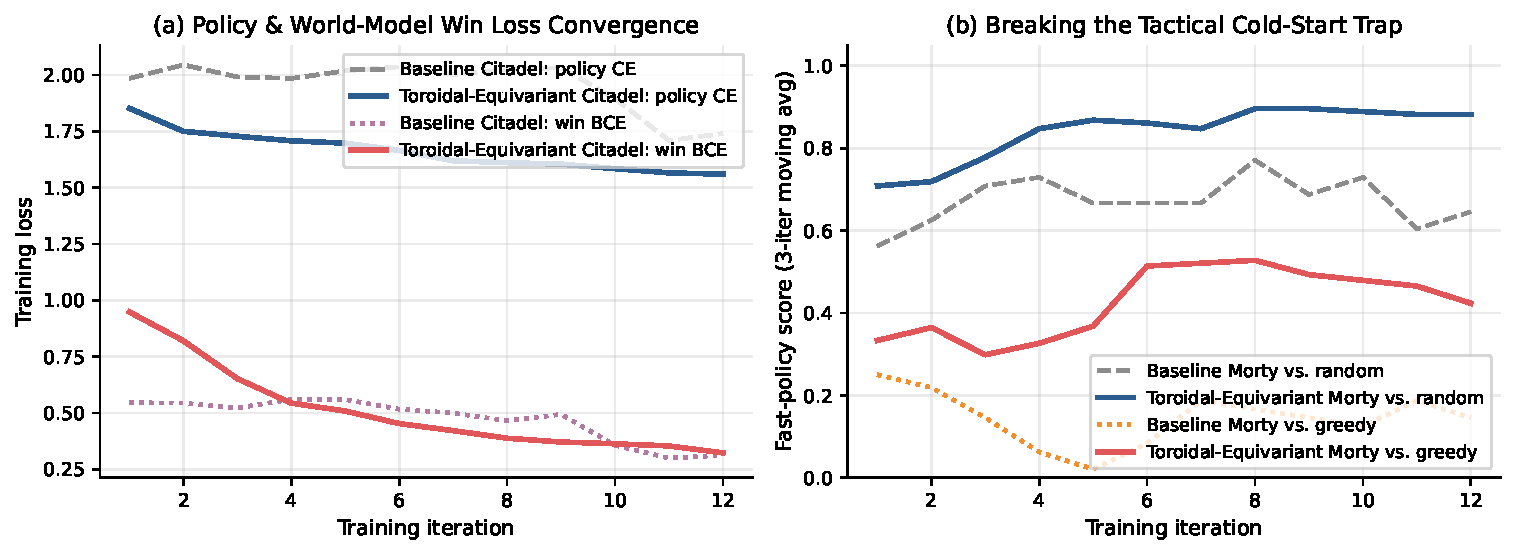
\includegraphics[width=\textwidth]{figures/fig4_architecture_comparison.pdf}
    \caption{\textbf{Breaking the tactical cold-start trap (\S\ref{sec:citadel}).} (a) Policy cross-entropy and world-model win binary cross-entropy across iterations for Baseline Citadel vs.\ Toroidal-Equivariant Citadel v2. (b) Fast-policy (\texttt{morty}) score against \texttt{random} and \texttt{greedy} opponents during training.}
    \label{fig:arch}
\end{figure}

\begin{figure}[t]
    \centering
    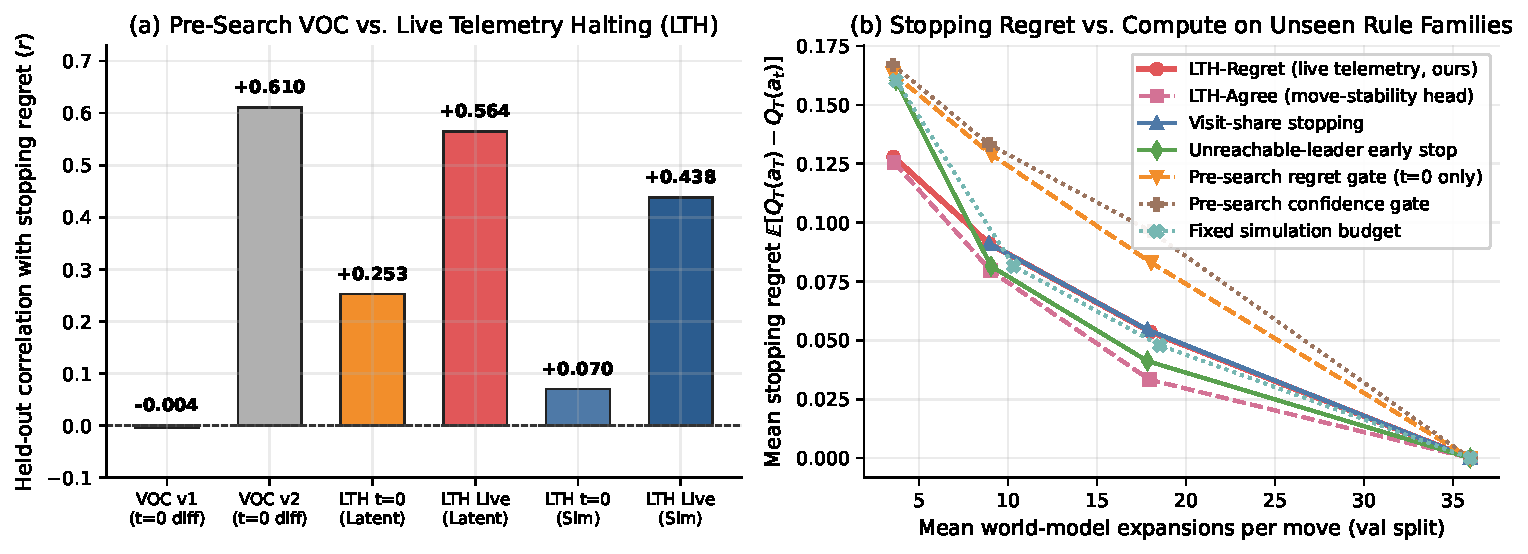
\includegraphics[width=\textwidth]{figures/fig1_halting_diagnosis.pdf}
    \caption{\textbf{Why pre-search VOC fails and why Mr.\ Meeseeks succeeds (\S\ref{sec:meeseeks}).} (a) Held-out correlation $r$ between predicted and actual stopping regret: pre-search features ($t=0$) carry weak signal, whereas live in-search telemetry ($t>0$) achieves strong positive correlation on both latent and simulator search traces. (b) Offline validation stopping regret $\mathbb{E}[Q_T(a_T) - Q_T(a_t)]$ vs.\ mean expansions per move across halting rules.}
    \label{fig:halting}
\end{figure}

\begin{figure}[t]
    \centering
    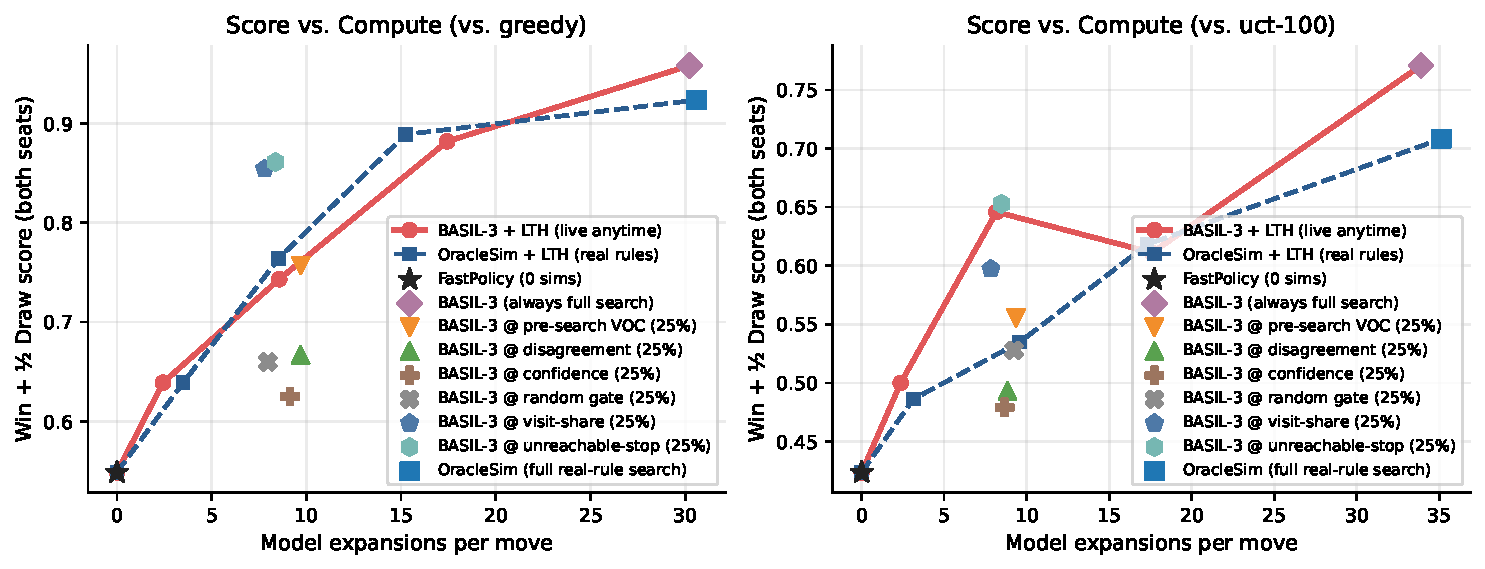
\includegraphics[width=\textwidth]{figures/fig2_pareto_compute.pdf}
    \caption{\textbf{Online game-play score vs.\ compute Pareto frontier} on unseen rule families, comparing \texttt{morty} ($0$ expansions), \texttt{Citadel+Meeseeks}, pre-search gates (\texttt{voc}, \texttt{disagreement}, \texttt{confidence}, \texttt{random}), anytime baselines (\texttt{share}, \texttt{unreach}), and \texttt{Oracle+Meeseeks}.}
    \label{fig:pareto}
\end{figure}

\begin{figure}[t]
    \centering
    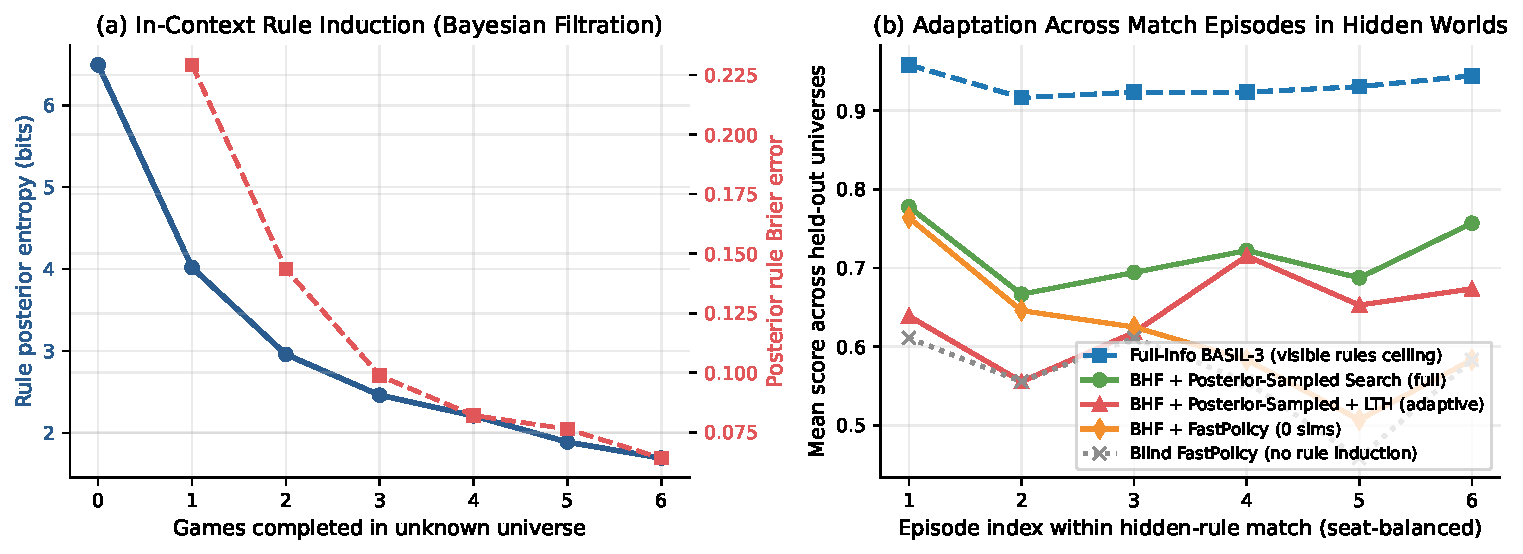
\includegraphics[width=\textwidth]{figures/fig3_cronenberg_cfc.pdf}
    \caption{\textbf{Cronenberg Mode: adaptation in hidden-rule universes (\S\ref{sec:cronenberg}).} (a) Exact Bayesian rule posterior entropy $H(P_t)$ (bits) and rule marginal Brier error across a 6-episode match in unseen universes. (b) Mean game score by episode index comparing blind play, Central Finite Curve + fast policy, Multiverse Thompson Search, and adaptive Meeseeks halting.}
    \label{fig:cronenberg}
\end{figure}

% Auto-generated by basil3.make_paper_figures -- do not edit by hand.
\begin{table}[t]
\centering
\small
\caption{\textbf{Halting calibration and stopping-regret accuracy} across seeds on held-out rule families. Live Telemetry Halting (LTH) achieves strong positive correlation with true stopping regret once in-search telemetry ($t>0$) is observed, yielding lower stopping regret and higher final-move agreement at matched $25\%$ compute budget.}
\label{tab:halting}
\begin{tabular}{lcccc}
\toprule
Halting Policy (@ $25\%$ Budget) & Regret Corr.\ $r$ ($t>0$) & Mean Exps/Move & Stopping Regret $\downarrow$ & Final-Move Agreement $\uparrow$ \\
\midrule
\textbf{Live Telemetry Halting (LTH-Regret, ours)} & $+0.564$ & $8.9$ & $0.0911$ & $74.7\%$ \\
\textbf{Live Telemetry Halting (LTH-Agree, ours)} & $---$ & $9.0$ & $0.0797$ & $76.3\%$ \\
Visit-share threshold ($s_{\text{top}} \ge \tau$) & $---$ & $8.9$ & $0.0911$ & $73.3\%$ \\
Unreachable-leader early stop & $---$ & $9.1$ & $0.0815$ & $75.3\%$ \\
Pre-search regret gate ($t=0$ only) & $+0.253$ & $9.1$ & $0.1288$ & $70.3\%$ \\
Pre-search policy-entropy gate & $---$ & $9.0$ & $0.1332$ & $70.3\%$ \\
Fixed simulation budget & $---$ & $10.3$ & $0.0815$ & $75.3\%$ \\
\bottomrule
\end{tabular}
\end{table}

\begin{table}[t]
\centering
\small
\caption{\textbf{Online game-play performance on unseen validation rule families} (paired evaluation across both seats, reporting mean score $\text{win} + \tfrac{1}{2}\text{draw}$, $95\%$ bootstrap CI over universes, paired $\Delta$ vs.\ \texttt{FastPolicy}, and model expansions per move).}
\label{tab:online}
\begin{tabular}{llcccc}
\toprule
Agent & Opponent & Score & $95\%$ CI & $\Delta$ vs.\ \texttt{FastPolicy} & Exps/Move \\
\midrule
FastPolicy ($0$ sims) & \texttt{greedy} & $0.549$ & $[0.347, 0.750]$ & $---$ & $0.0$ \\
BASIL-3 (Full Search) & \texttt{greedy} & $0.958$ & $[0.875, 1.000]$ & $+0.410$ & $30.2$ \\
BASIL-3 + LTH-Regret ($10\%$) & \texttt{greedy} & $0.639$ & $[0.438, 0.833]$ & $+0.090$ & $2.4$ \\
BASIL-3 + LTH-Regret ($25\%$) & \texttt{greedy} & $0.743$ & $[0.597, 0.875]$ & $+0.194$ & $8.6$ \\
BASIL-3 + LTH-Regret ($50\%$) & \texttt{greedy} & $0.882$ & $[0.757, 0.979]$ & $+0.333$ & $17.4$ \\
BASIL-3 + LTH-Agree ($25\%$) & \texttt{greedy} & $0.785$ & $[0.632, 0.917]$ & $+0.236$ & $7.2$ \\
BASIL-3 + Pre-Regret ($25\%$) & \texttt{greedy} & $0.646$ & $[0.465, 0.833]$ & $+0.097$ & $7.3$ \\
BASIL-3 + VisitShare ($25\%$) & \texttt{greedy} & $0.854$ & $[0.715, 0.965]$ & $+0.306$ & $7.8$ \\
BASIL-3 + UnreachStop ($25\%$) & \texttt{greedy} & $0.861$ & $[0.750, 0.958]$ & $+0.312$ & $8.4$ \\
BASIL-3 + Pre-VOC ($25\%$) & \texttt{greedy} & $0.757$ & $[0.562, 0.938]$ & $+0.208$ & $9.7$ \\
BASIL-3 + Disagreement ($25\%$) & \texttt{greedy} & $0.667$ & $[0.479, 0.847]$ & $+0.118$ & $9.7$ \\
BASIL-3 + Confidence ($25\%$) & \texttt{greedy} & $0.625$ & $[0.403, 0.833]$ & $+0.076$ & $9.1$ \\
BASIL-3 + RandomGate ($25\%$) & \texttt{greedy} & $0.660$ & $[0.458, 0.847]$ & $+0.111$ & $8.0$ \\
OracleSim (Full Search) & \texttt{greedy} & $0.924$ & $[0.826, 1.000]$ & $+0.375$ & $30.6$ \\
OracleSim + LTH-Regret ($10\%$) & \texttt{greedy} & $0.639$ & $[0.458, 0.826]$ & $+0.090$ & $3.5$ \\
OracleSim + LTH-Regret ($25\%$) & \texttt{greedy} & $0.764$ & $[0.618, 0.889]$ & $+0.215$ & $8.5$ \\
OracleSim + LTH-Regret ($50\%$) & \texttt{greedy} & $0.889$ & $[0.778, 0.979]$ & $+0.340$ & $15.2$ \\
FastPolicy ($0$ sims) & \texttt{uct-100} & $0.424$ & $[0.208, 0.639]$ & $---$ & $0.0$ \\
BASIL-3 (Full Search) & \texttt{uct-100} & $0.771$ & $[0.639, 0.889]$ & $+0.347$ & $33.9$ \\
BASIL-3 + LTH-Regret ($10\%$) & \texttt{uct-100} & $0.500$ & $[0.291, 0.722]$ & $+0.076$ & $2.4$ \\
BASIL-3 + LTH-Regret ($25\%$) & \texttt{uct-100} & $0.646$ & $[0.417, 0.854]$ & $+0.222$ & $8.2$ \\
BASIL-3 + LTH-Regret ($50\%$) & \texttt{uct-100} & $0.611$ & $[0.375, 0.812]$ & $+0.188$ & $17.6$ \\
BASIL-3 + LTH-Agree ($25\%$) & \texttt{uct-100} & $0.583$ & $[0.382, 0.778]$ & $+0.160$ & $7.9$ \\
BASIL-3 + Pre-Regret ($25\%$) & \texttt{uct-100} & $0.542$ & $[0.306, 0.764]$ & $+0.118$ & $8.1$ \\
BASIL-3 + VisitShare ($25\%$) & \texttt{uct-100} & $0.597$ & $[0.375, 0.806]$ & $+0.174$ & $7.8$ \\
BASIL-3 + UnreachStop ($25\%$) & \texttt{uct-100} & $0.653$ & $[0.465, 0.833]$ & $+0.229$ & $8.5$ \\
BASIL-3 + Pre-VOC ($25\%$) & \texttt{uct-100} & $0.556$ & $[0.354, 0.764]$ & $+0.132$ & $9.4$ \\
BASIL-3 + Disagreement ($25\%$) & \texttt{uct-100} & $0.493$ & $[0.292, 0.708]$ & $+0.069$ & $8.8$ \\
BASIL-3 + Confidence ($25\%$) & \texttt{uct-100} & $0.479$ & $[0.250, 0.701]$ & $+0.056$ & $8.7$ \\
BASIL-3 + RandomGate ($25\%$) & \texttt{uct-100} & $0.528$ & $[0.292, 0.750]$ & $+0.104$ & $9.2$ \\
OracleSim (Full Search) & \texttt{uct-100} & $0.708$ & $[0.542, 0.861]$ & $+0.285$ & $35.1$ \\
OracleSim + LTH-Regret ($10\%$) & \texttt{uct-100} & $0.486$ & $[0.264, 0.708]$ & $+0.062$ & $3.1$ \\
OracleSim + LTH-Regret ($25\%$) & \texttt{uct-100} & $0.535$ & $[0.306, 0.750]$ & $+0.111$ & $9.6$ \\
OracleSim + LTH-Regret ($50\%$) & \texttt{uct-100} & $0.618$ & $[0.430, 0.806]$ & $+0.194$ & $17.3$ \\
\bottomrule
\end{tabular}
\end{table}

\begin{table}[t]
\centering
\small
\caption{\textbf{Hidden-Rule Regime multi-episode adaptation} across unseen universes. Exact Bayesian Hypothesis Filtration (BHF) reduces rule posterior entropy from $6.49$ bits ($90.0$ candidate universes on average) at the start of Episode 1 to $1.69$ bits by the end of Episode 6.}
\label{tab:cronenberg}
\begin{tabular}{lcccc}
\toprule
Hidden-Rule Agent Architecture & Ep.\ 1--2 Score & Ep.\ 5--6 Score & Mean Match Score & Mean Exps/Move \\
\midrule
Blind FastPolicy (no rule induction) & $0.555$ & $0.583$ & $0.565$ & $0.0$ \\
BHF + FastPolicy ($0$ sims) & $0.646$ & $0.583$ & $0.604$ & $0.0$ \\
\textbf{BHF + Posterior-Sampled Search + LTH (adaptive)} & $0.556$ & $0.674$ & $0.648$ & $19.6$ \\
\textbf{BHF + Posterior-Sampled Search (full)} & $0.667$ & $0.757$ & $0.715$ & $38.3$ \\
Full-Info BASIL-3 (visible rules ceiling) & $0.917$ & $0.945$ & $0.928$ & $30.8$ \\
\bottomrule
\end{tabular}
\end{table}

\begin{table}[t]
\centering
\small
\caption{\textbf{One-shot preregistered test-split evaluation} on held-out rule families (cryptographically locked prior to test evaluation, 3 seeds $\times$ both seats).}
\label{tab:test_online}
\begin{tabular}{llcccc}
\toprule
Agent & Opponent & Test Score & $95\%$ CI & $\Delta$ vs.\ \texttt{FastPolicy} & Exps/Move \\
\midrule
FastPolicy ($0$ sims) & \texttt{greedy} & $0.597$ & $[0.417, 0.764]$ & $---$ & $0.0$ \\
BASIL-3 (Full Search) & \texttt{greedy} & $0.938$ & $[0.833, 1.000]$ & $+0.340$ & $34.1$ \\
BASIL-3 + LTH-Regret ($10\%$) & \texttt{greedy} & $0.646$ & $[0.451, 0.833]$ & $+0.049$ & $3.8$ \\
BASIL-3 + LTH-Regret ($25\%$) & \texttt{greedy} & $0.750$ & $[0.597, 0.889]$ & $+0.153$ & $10.8$ \\
BASIL-3 + LTH-Regret ($50\%$) & \texttt{greedy} & $0.778$ & $[0.625, 0.917]$ & $+0.181$ & $20.1$ \\
BASIL-3 + LTH-Agree ($25\%$) & \texttt{greedy} & $0.764$ & $[0.597, 0.910]$ & $+0.167$ & $10.9$ \\
BASIL-3 + Pre-Regret ($25\%$) & \texttt{greedy} & $0.681$ & $[0.500, 0.847]$ & $+0.083$ & $9.2$ \\
BASIL-3 + VisitShare ($25\%$) & \texttt{greedy} & $0.806$ & $[0.639, 0.931]$ & $+0.208$ & $9.8$ \\
BASIL-3 + UnreachStop ($25\%$) & \texttt{greedy} & $0.743$ & $[0.548, 0.917]$ & $+0.146$ & $9.1$ \\
BASIL-3 + Pre-VOC ($25\%$) & \texttt{greedy} & $0.743$ & $[0.583, 0.896]$ & $+0.146$ & $10.7$ \\
BASIL-3 + Disagreement ($25\%$) & \texttt{greedy} & $0.604$ & $[0.403, 0.792]$ & $+0.007$ & $7.2$ \\
BASIL-3 + Confidence ($25\%$) & \texttt{greedy} & $0.688$ & $[0.542, 0.833]$ & $+0.090$ & $13.8$ \\
BASIL-3 + RandomGate ($25\%$) & \texttt{greedy} & $0.639$ & $[0.417, 0.847]$ & $+0.042$ & $8.2$ \\
OracleSim (Full Search) & \texttt{greedy} & $0.903$ & $[0.784, 1.000]$ & $+0.306$ & $33.7$ \\
OracleSim + LTH-Regret ($10\%$) & \texttt{greedy} & $0.604$ & $[0.403, 0.792]$ & $+0.007$ & $4.0$ \\
OracleSim + LTH-Regret ($25\%$) & \texttt{greedy} & $0.771$ & $[0.583, 0.931]$ & $+0.174$ & $9.6$ \\
OracleSim + LTH-Regret ($50\%$) & \texttt{greedy} & $0.847$ & $[0.708, 0.958]$ & $+0.250$ & $18.1$ \\
FastPolicy ($0$ sims) & \texttt{uct-100} & $0.486$ & $[0.292, 0.667]$ & $---$ & $0.0$ \\
BASIL-3 (Full Search) & \texttt{uct-100} & $0.722$ & $[0.542, 0.875]$ & $+0.236$ & $35.8$ \\
BASIL-3 + LTH-Regret ($10\%$) & \texttt{uct-100} & $0.542$ & $[0.375, 0.708]$ & $+0.056$ & $3.7$ \\
BASIL-3 + LTH-Regret ($25\%$) & \texttt{uct-100} & $0.639$ & $[0.458, 0.819]$ & $+0.153$ & $10.0$ \\
BASIL-3 + LTH-Regret ($50\%$) & \texttt{uct-100} & $0.688$ & $[0.500, 0.854]$ & $+0.201$ & $18.8$ \\
BASIL-3 + LTH-Agree ($25\%$) & \texttt{uct-100} & $0.681$ & $[0.521, 0.833]$ & $+0.194$ & $10.5$ \\
BASIL-3 + Pre-Regret ($25\%$) & \texttt{uct-100} & $0.556$ & $[0.361, 0.736]$ & $+0.069$ & $8.4$ \\
BASIL-3 + VisitShare ($25\%$) & \texttt{uct-100} & $0.688$ & $[0.458, 0.861]$ & $+0.201$ & $8.9$ \\
BASIL-3 + UnreachStop ($25\%$) & \texttt{uct-100} & $0.701$ & $[0.542, 0.854]$ & $+0.215$ & $9.0$ \\
BASIL-3 + Pre-VOC ($25\%$) & \texttt{uct-100} & $0.632$ & $[0.403, 0.847]$ & $+0.146$ & $9.9$ \\
BASIL-3 + Disagreement ($25\%$) & \texttt{uct-100} & $0.528$ & $[0.333, 0.708]$ & $+0.042$ & $7.7$ \\
BASIL-3 + Confidence ($25\%$) & \texttt{uct-100} & $0.507$ & $[0.277, 0.736]$ & $+0.021$ & $11.5$ \\
BASIL-3 + RandomGate ($25\%$) & \texttt{uct-100} & $0.549$ & $[0.375, 0.722]$ & $+0.062$ & $6.9$ \\
OracleSim (Full Search) & \texttt{uct-100} & $0.708$ & $[0.542, 0.847]$ & $+0.222$ & $36.0$ \\
OracleSim + LTH-Regret ($10\%$) & \texttt{uct-100} & $0.514$ & $[0.333, 0.681]$ & $+0.028$ & $3.2$ \\
OracleSim + LTH-Regret ($25\%$) & \texttt{uct-100} & $0.653$ & $[0.444, 0.833]$ & $+0.167$ & $9.7$ \\
OracleSim + LTH-Regret ($50\%$) & \texttt{uct-100} & $0.708$ & $[0.535, 0.868]$ & $+0.222$ & $18.1$ \\
\bottomrule
\end{tabular}
\end{table}


\section{Conclusion}
We have shown that making adaptive test-time imagination work on unseen games requires aligning three layers of the agent: (1) an equivariant, rule-preserving world model that transfers across board topologies and learns from contrastive counterfactual action probes; (2) an anytime halting policy (Mr.\ Meeseeks) trained on low-variance self-supervised search traces and conditioned on live tree telemetry rather than pre-search guesses; and (3) in-context Bayesian rule induction over the Central Finite Curve when the laws of the environment are hidden. All code, preregistration hashes, checkpoints, and evaluation scripts are openly available in the repository.

\bibliographystyle{plainnat}
\bibliography{references}

\end{document}
